\documentclass[UTF8,11pt]{ctexart}
\usepackage[a4paper,margin=22mm]{geometry}
\usepackage{amsmath,amssymb,bm,graphicx,adjustbox,fvextra,longtable,array}
\xeCJKDeclareCharClass{CJK}{"2160 -> "217F, "2460 -> "249B, "2200 -> "22FF}
\newcommand{\fitmath}[1]{\begin{adjustbox}{max width=\linewidth}$\displaystyle #1$\end{adjustbox}}
\setlength{\parindent}{0pt}\setlength{\parskip}{.65em}\renewcommand{\arraystretch}{1.3}
\sloppy\allowdisplaybreaks
\begin{document}
\section*{2022 年计算机统考 408 · 真题}
\subsection*{2022年全国硕士研究生入学统一考试}

\subsection*{计算机学科专业基础综合试题}

\subsection*{一、单项选择题（1～40小题，每小题2分，共80分。下列每小题给出的四个选项中，只有一项符合题目要求）}

1．下列程序段的时间复杂度是\_\_\_\_\_\_。


\begin{Verbatim}[breaklines,breakanywhere,fontsize=\small]
int sum = 0;
for (int i = 1; i < n; i *= 2)
    for (int j = 0; j < i; j++)
        sum++;
\end{Verbatim}

\begin{center}\begin{tabular}{>{\raggedright\arraybackslash}p{\dimexpr(\linewidth-8\tabcolsep)/4\relax}>{\raggedright\arraybackslash}p{\dimexpr(\linewidth-8\tabcolsep)/4\relax}>{\raggedright\arraybackslash}p{\dimexpr(\linewidth-8\tabcolsep)/4\relax}>{\raggedright\arraybackslash}p{\dimexpr(\linewidth-8\tabcolsep)/4\relax}}
\textbf{A.} \(\displaystyle O(\log n)\) & \textbf{B.} \(\displaystyle O(n)\) & \textbf{C.} \(\displaystyle O(n\log n)\) & \textbf{D.} \(\displaystyle O(n^2)\)\\[.35em]\end{tabular}\end{center}

2．给定有限符号集S，in 和out 均为S 中所有元素的任意排列。对于初始为空的栈ST，下列叙述中，正确的是\_\_\_\_\_\_。


\begin{center}\begin{tabular}{>{\raggedright\arraybackslash}p{\dimexpr(\linewidth-4\tabcolsep)/2\relax}>{\raggedright\arraybackslash}p{\dimexpr(\linewidth-4\tabcolsep)/2\relax}}
\textbf{A.} 若in 是ST 的入栈序列，则不能判断out 是否为其可能的出栈序列 & \textbf{B.} 若out 是ST 的出栈序列，则不能判断in 是否为其可能的入栈序列\\[.35em]
\textbf{C.} 若in 是ST 的入栈序列，out 是对应in 的出栈序列，则in 与out 一定不同 & \textbf{D.} 若in 是ST 的入栈序列，out 是对应的出栈序列，则in 与out 可能互为倒序\\[.35em]\end{tabular}\end{center}

3．若结点p 与q 在二叉树T 的中序遍历序列中相邻，且p 在q 之前，则下列p 与q 的关系中，不． 可能的是\_\_\_\_\_\_。 I. q 是p 的双亲 II. q 是p 的右孩子 III. q 是p 的右兄弟 IV. q 是p 的双亲的双亲


\begin{center}\begin{tabular}{>{\raggedright\arraybackslash}p{\dimexpr(\linewidth-8\tabcolsep)/4\relax}>{\raggedright\arraybackslash}p{\dimexpr(\linewidth-8\tabcolsep)/4\relax}>{\raggedright\arraybackslash}p{\dimexpr(\linewidth-8\tabcolsep)/4\relax}>{\raggedright\arraybackslash}p{\dimexpr(\linewidth-8\tabcolsep)/4\relax}}
\textbf{A.} 仅I & \textbf{B.} 仅III & \textbf{C.} 仅II、III & \textbf{D.} 仅II、IV\\[.35em]\end{tabular}\end{center}

4．若三叉树T 中有244 个结点（叶结点的高度为1），则T 的高度至少是\_\_\_\_\_\_。


\begin{center}\begin{tabular}{>{\raggedright\arraybackslash}p{\dimexpr(\linewidth-8\tabcolsep)/4\relax}>{\raggedright\arraybackslash}p{\dimexpr(\linewidth-8\tabcolsep)/4\relax}>{\raggedright\arraybackslash}p{\dimexpr(\linewidth-8\tabcolsep)/4\relax}>{\raggedright\arraybackslash}p{\dimexpr(\linewidth-8\tabcolsep)/4\relax}}
\textbf{A.} 8 & \textbf{B.} 7 & \textbf{C.} 6 & \textbf{D.} 5\\[.35em]\end{tabular}\end{center}

5．对任意给定的含n（n > 2）个字符的有限集S，用二叉树表示S 的哈夫曼编码集和定长编码集， 分别得到二叉树T1 和T2。下列叙述中，正确的是\_\_\_\_\_\_。


\begin{center}\begin{tabular}{>{\raggedright\arraybackslash}p{\dimexpr(\linewidth-4\tabcolsep)/2\relax}>{\raggedright\arraybackslash}p{\dimexpr(\linewidth-4\tabcolsep)/2\relax}}
\textbf{A.} T1 与T2 的结点数相同 & \textbf{B.} T1 的高度大于T2 的高度\\[.35em]
\textbf{C.} 出现频次不同的字符在T1 中处于不同的层 & \textbf{D.} 出现频次不同的字符在T2 中处于相同的层\\[.35em]\end{tabular}\end{center}

6．对于无向图G = (V, E)，下列选项中，正确的是\_\_\_\_\_\_。


\begin{center}\begin{tabular}{>{\raggedright\arraybackslash}p{\dimexpr(\linewidth-4\tabcolsep)/2\relax}>{\raggedright\arraybackslash}p{\dimexpr(\linewidth-4\tabcolsep)/2\relax}}
\textbf{A.} 当| V | > | E |时，G 一定是连通的 & \textbf{B.} 当| V | < | E |时，G 一定是连通的\\[.35em]
\textbf{C.} 当| V | = | E | – 1 时，G 一定是不连通的 & \textbf{D.} 当| V | > | E | + 1 时，G 一定是不连通的\\[.35em]\end{tabular}\end{center}

7．下图是一个有10 个活动的AOE 网，时间余量最大的活动是\_\_\_\_\_\_。


\begin{center}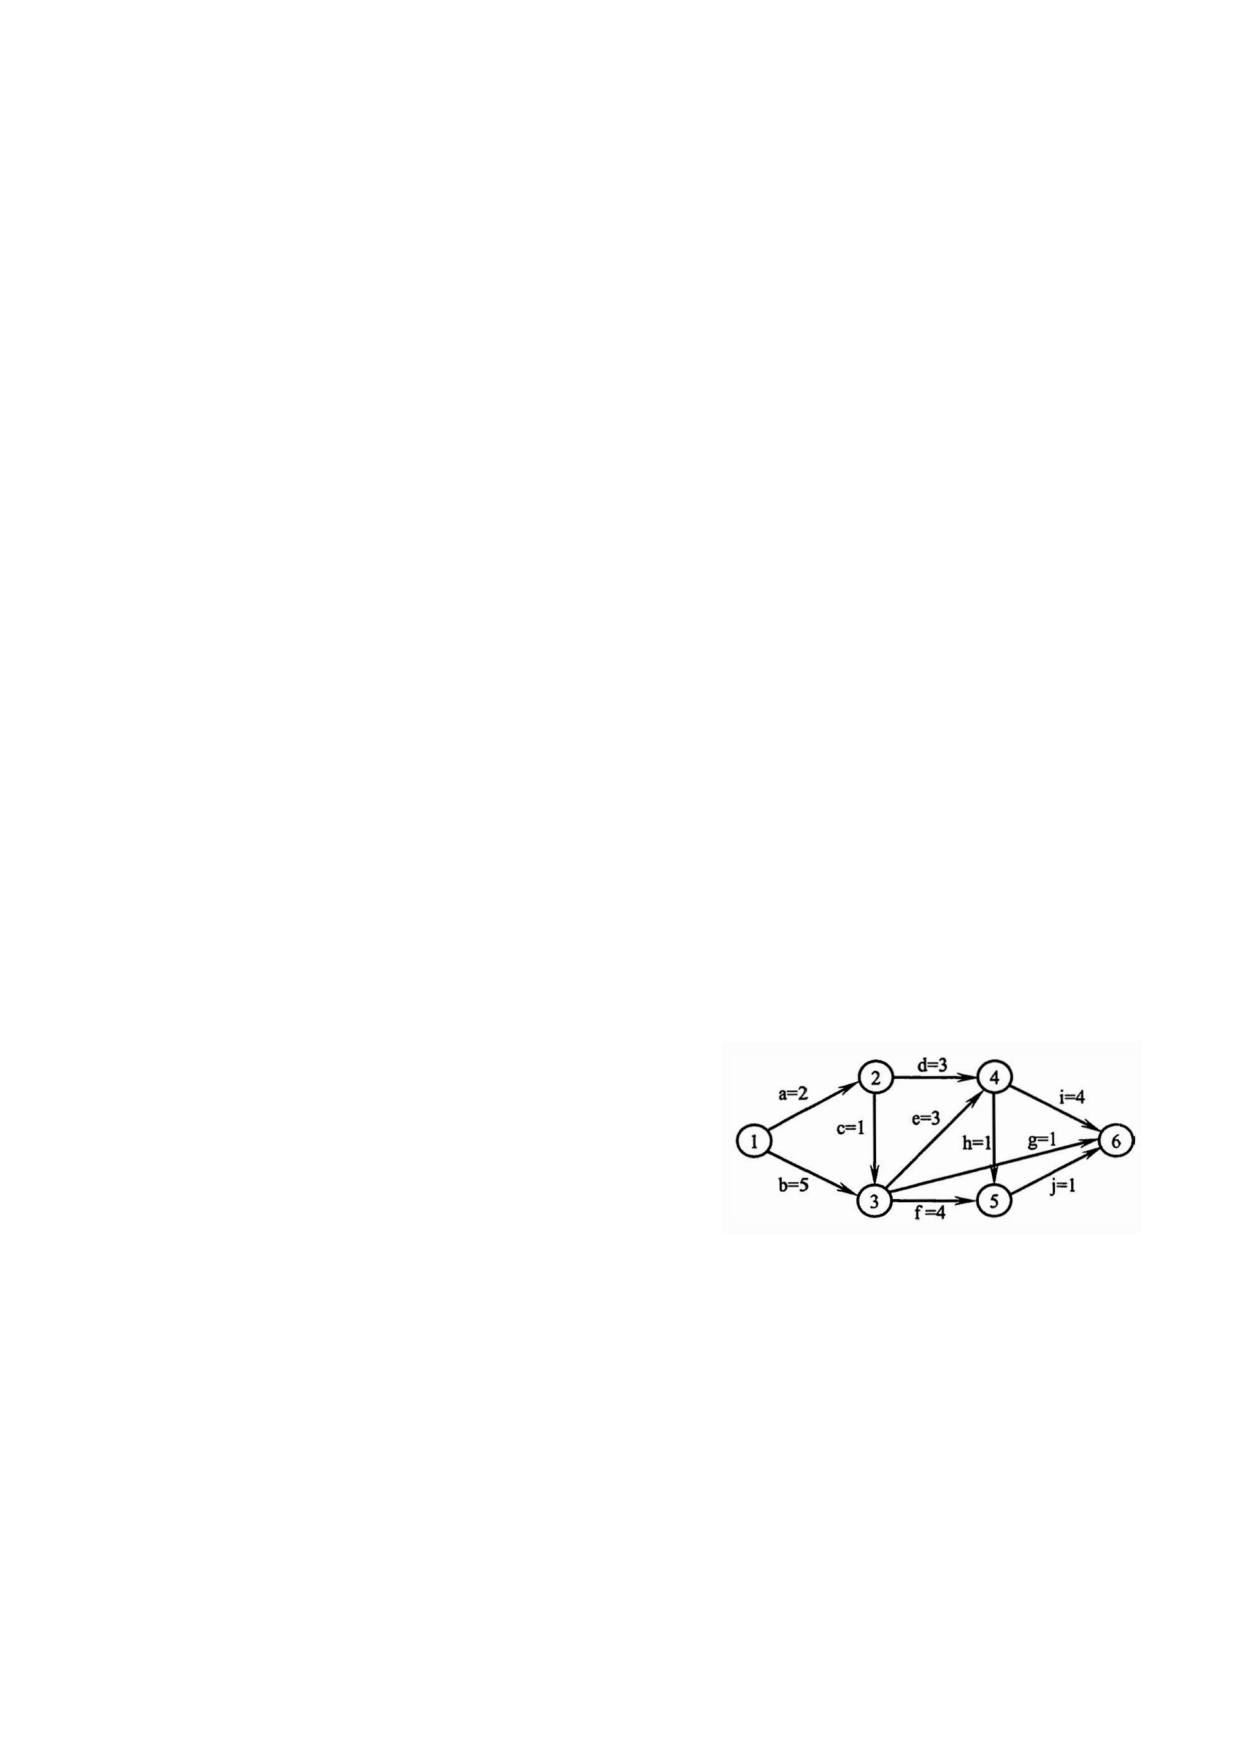
\includegraphics[width=.65\linewidth,height=.4\textheight,keepaspectratio]{../assets/figures/2022-questions-p001-b012.pdf}\end{center}

\begin{center}\begin{tabular}{>{\raggedright\arraybackslash}p{\dimexpr(\linewidth-8\tabcolsep)/4\relax}>{\raggedright\arraybackslash}p{\dimexpr(\linewidth-8\tabcolsep)/4\relax}>{\raggedright\arraybackslash}p{\dimexpr(\linewidth-8\tabcolsep)/4\relax}>{\raggedright\arraybackslash}p{\dimexpr(\linewidth-8\tabcolsep)/4\relax}}
\textbf{A.} c & \textbf{B.} g & \textbf{C.} h & \textbf{D.} j\\[.35em]\end{tabular}\end{center}

8．在下图所示的5 阶B 树T 中，删除关键字260 之后需要进行必要的调整，得到新的B 树T1。下列选项中，不可能是T1 根结点中关键字序列的是\_\_\_\_\_\_。


\begin{center}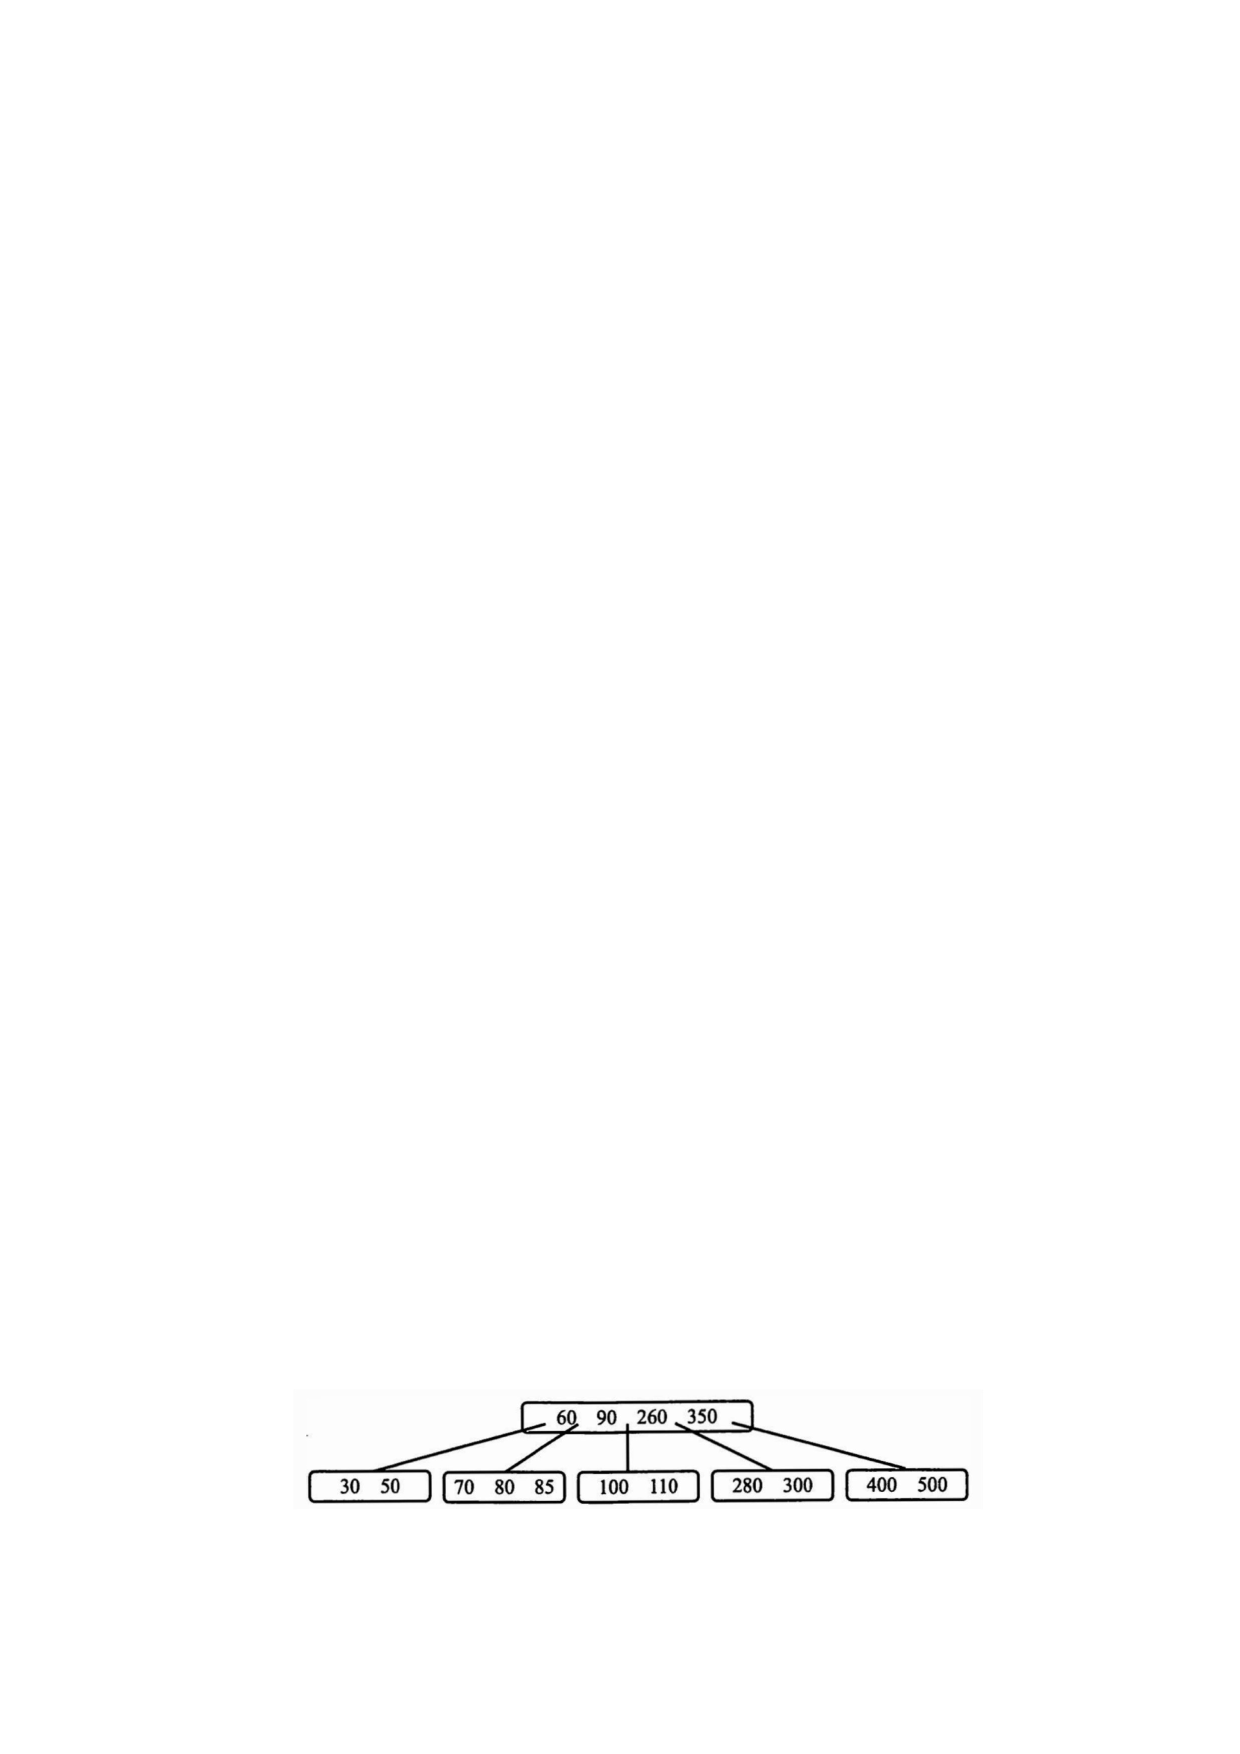
\includegraphics[width=.65\linewidth,height=.4\textheight,keepaspectratio]{../assets/figures/2022-questions-p001-b015.pdf}\end{center}

\begin{center}\begin{tabular}{>{\raggedright\arraybackslash}p{\dimexpr(\linewidth-8\tabcolsep)/4\relax}>{\raggedright\arraybackslash}p{\dimexpr(\linewidth-8\tabcolsep)/4\relax}>{\raggedright\arraybackslash}p{\dimexpr(\linewidth-8\tabcolsep)/4\relax}>{\raggedright\arraybackslash}p{\dimexpr(\linewidth-8\tabcolsep)/4\relax}}
\textbf{A.} 60, 90, 280 & \textbf{B.} 60, 90, 350 & \textbf{C.} 60, 85, 110, 350 & \textbf{D.} 60, 90, 110, 350\\[.35em]\end{tabular}\end{center}

9．下列因素中，影响散列（哈希）方法平均查找长度的是\_\_\_\_\_\_。 I. 装填因子 II. 散列函数 III. 冲突解决策略


\begin{center}\begin{tabular}{>{\raggedright\arraybackslash}p{\dimexpr(\linewidth-8\tabcolsep)/4\relax}>{\raggedright\arraybackslash}p{\dimexpr(\linewidth-8\tabcolsep)/4\relax}>{\raggedright\arraybackslash}p{\dimexpr(\linewidth-8\tabcolsep)/4\relax}>{\raggedright\arraybackslash}p{\dimexpr(\linewidth-8\tabcolsep)/4\relax}}
\textbf{A.} 仅I、II & \textbf{B.} 仅I、III & \textbf{C.} 仅II、III & \textbf{D.} I、II、III\\[.35em]\end{tabular}\end{center}

10．使用二路归并排序对含n 个元素的数组M 进行排序时，二路归并操作的功能是\_\_\_\_\_\_。


\begin{center}\begin{tabular}{>{\raggedright\arraybackslash}p{\dimexpr(\linewidth-4\tabcolsep)/2\relax}>{\raggedright\arraybackslash}p{\dimexpr(\linewidth-4\tabcolsep)/2\relax}}
\textbf{A.} 将两个有序表合并为一个新的有序表 & \textbf{B.} 将M 划分为两部分，两部分的元素个数大致相等\\[.35em]
\textbf{C.} 将M 划分为n 个部分，每个部分中仅含有一个元素 & \textbf{D.} 将M 划分为两部分，一部分元素的值均小于另一部分元素的值\\[.35em]\end{tabular}\end{center}

11．对数据进行排序时，若采用直接插入排序而不采用快速排序，则可能的原因是\_\_\_\_\_\_。 I. 大部分元素己有序 II. 待排序元素数量很少 III. 要求空间复杂度为O(1) IV. 要求排序算法是稳定的


\begin{center}\begin{tabular}{>{\raggedright\arraybackslash}p{\dimexpr(\linewidth-8\tabcolsep)/4\relax}>{\raggedright\arraybackslash}p{\dimexpr(\linewidth-8\tabcolsep)/4\relax}>{\raggedright\arraybackslash}p{\dimexpr(\linewidth-8\tabcolsep)/4\relax}>{\raggedright\arraybackslash}p{\dimexpr(\linewidth-8\tabcolsep)/4\relax}}
\textbf{A.} 仅I、II & \textbf{B.} 仅III、IV & \textbf{C.} 仅I、II、IV & \textbf{D.} I、II、III、IV\\[.35em]\end{tabular}\end{center}

12．某计算机主频为1GHz，程序p 运行过程中，共执行了10000 条指令，其中，80\%的指令执行平均需1 个时钟周期，20\%的指令执行平均需10 个时钟周期。程序P 的平均CPI 和CPU 执行时间分别是\_\_\_\_\_\_。


\begin{center}\begin{tabular}{>{\raggedright\arraybackslash}p{\dimexpr(\linewidth-8\tabcolsep)/4\relax}>{\raggedright\arraybackslash}p{\dimexpr(\linewidth-8\tabcolsep)/4\relax}>{\raggedright\arraybackslash}p{\dimexpr(\linewidth-8\tabcolsep)/4\relax}>{\raggedright\arraybackslash}p{\dimexpr(\linewidth-8\tabcolsep)/4\relax}}
\textbf{A.} 2.\allowbreak{}8，\(\displaystyle 28\,\mu\mathrm{s}\) & \textbf{B.} 28, \(\displaystyle 28\,\mu\mathrm{s}\) & \textbf{C.} 2.\allowbreak{}8, 28ms & \textbf{D.} 28, 28ms\\[.35em]\end{tabular}\end{center}

13．32位补码所能表示的整数范围是\_\_\_\_\_\_。


\begin{center}\begin{tabular}{>{\raggedright\arraybackslash}p{\dimexpr(\linewidth-8\tabcolsep)/4\relax}>{\raggedright\arraybackslash}p{\dimexpr(\linewidth-8\tabcolsep)/4\relax}>{\raggedright\arraybackslash}p{\dimexpr(\linewidth-8\tabcolsep)/4\relax}>{\raggedright\arraybackslash}p{\dimexpr(\linewidth-8\tabcolsep)/4\relax}}
\textbf{A.} \(\displaystyle -2^{32}\sim2^{31}-1\) & \textbf{B.} \(\displaystyle -2^{31}\sim2^{31}-1\) & \textbf{C.} \(\displaystyle -2^{32}\sim2^{32}-1\) & \textbf{D.} \(\displaystyle -2^{31}\sim2^{32}-1\)\\[.35em]\end{tabular}\end{center}

14．－0.4375 的IEEE 754 单精度浮点数表示为\_\_\_\_\_\_。


\begin{center}\begin{tabular}{>{\raggedright\arraybackslash}p{\dimexpr(\linewidth-8\tabcolsep)/4\relax}>{\raggedright\arraybackslash}p{\dimexpr(\linewidth-8\tabcolsep)/4\relax}>{\raggedright\arraybackslash}p{\dimexpr(\linewidth-8\tabcolsep)/4\relax}>{\raggedright\arraybackslash}p{\dimexpr(\linewidth-8\tabcolsep)/4\relax}}
\textbf{A.} BEE0 0000H & \textbf{B.} BF60 0000H & \textbf{C.} BF70 0000H & \textbf{D.} C0E0 0000H\\[.35em]\end{tabular}\end{center}

15．某计算机主存地址为24位，采用分页虚拟存储管理方式，虚拟地址空间大小为4GB，页大小为4KB，按字节编址。某进程的页表部分内容如下表所示。


\begin{center}\begin{adjustbox}{max width=\linewidth}\begin{tabular}{|>{\raggedright\arraybackslash}p{\dimexpr(\linewidth-6\tabcolsep-4\arrayrulewidth)/3\relax}|>{\raggedright\arraybackslash}p{\dimexpr(\linewidth-6\tabcolsep-4\arrayrulewidth)/3\relax}|>{\raggedright\arraybackslash}p{\dimexpr(\linewidth-6\tabcolsep-4\arrayrulewidth)/3\relax}|}\hline
虚页号 & 实页号（页框号） & 存在位\\\hline
82 & 024H & 0\\\hline
… & … & …\\\hline
129 & 180H & 1\\\hline
130 & 018H & 1\\\hline\end{tabular}\end{adjustbox}\end{center}

当CPU访问虚拟地址0008 2840H时，虚–实地址转换的结果是\_\_\_\_\_\_。


\begin{center}\begin{tabular}{>{\raggedright\arraybackslash}p{\dimexpr(\linewidth-4\tabcolsep)/2\relax}>{\raggedright\arraybackslash}p{\dimexpr(\linewidth-4\tabcolsep)/2\relax}}
\textbf{A.} 得到主存地址02 4840H & \textbf{B.} 得到主存地址18 0840H\\[.35em]
\textbf{C.} 得到主存地址01 8840H & \textbf{D.} 检测到缺页异常\\[.35em]\end{tabular}\end{center}

16．若计算机主存地址为32 位，按字节编址，某Cache 的数据区容量为32KB，主存块大小为64B， 采用8 路组相联映射方式，该Cache 中比较器的个数和位数分别为\_\_\_\_\_\_。


\begin{center}\begin{tabular}{>{\raggedright\arraybackslash}p{\dimexpr(\linewidth-8\tabcolsep)/4\relax}>{\raggedright\arraybackslash}p{\dimexpr(\linewidth-8\tabcolsep)/4\relax}>{\raggedright\arraybackslash}p{\dimexpr(\linewidth-8\tabcolsep)/4\relax}>{\raggedright\arraybackslash}p{\dimexpr(\linewidth-8\tabcolsep)/4\relax}}
\textbf{A.} 8, 20 & \textbf{B.} 8, 23 & \textbf{C.} 64, 20 & \textbf{D.} 64, 23\\[.35em]\end{tabular}\end{center}

17．某内存条包含8 个8192×8192×8 位的DRAM 芯片，按字节编址，支持突发（burst）传送方式，对应存储器总线宽度为64 位，每个DRAM 芯片内有一个行缓冲区（row buffer）。下列关于该内存条的叙述中，不正确的是\_\_\_\_\_\_。


\begin{center}\begin{tabular}{>{\raggedright\arraybackslash}p{\dimexpr(\linewidth-4\tabcolsep)/2\relax}>{\raggedright\arraybackslash}p{\dimexpr(\linewidth-4\tabcolsep)/2\relax}}
\textbf{A.} 内存条的容量为512MB & \textbf{B.} 采用多模块交叉编址方式\\[.35em]
\textbf{C.} 芯片的地址引脚为26 位 & \textbf{D.} 芯片内行缓冲有8192×8 位\\[.35em]\end{tabular}\end{center}

18．下列选项中，属于指令集体系结构（ISA）规定的内容是\_\_\_\_\_\_。 I. 指令字格式和指令类型 II. CPU 的时钟周期 III. 通用寄存器个数和位数 IV. 加法器的进位方式


\begin{center}\begin{tabular}{>{\raggedright\arraybackslash}p{\dimexpr(\linewidth-8\tabcolsep)/4\relax}>{\raggedright\arraybackslash}p{\dimexpr(\linewidth-8\tabcolsep)/4\relax}>{\raggedright\arraybackslash}p{\dimexpr(\linewidth-8\tabcolsep)/4\relax}>{\raggedright\arraybackslash}p{\dimexpr(\linewidth-8\tabcolsep)/4\relax}}
\textbf{A.} 仅I、II & \textbf{B.} 仅I、III & \textbf{C.} 仅II、IV & \textbf{D.} 仅I、III、IV\\[.35em]\end{tabular}\end{center}

19．设计某指令系统时，假设采用16 位定长指令字格式，操作码使用扩展编码方式，地址码为6 位，包含零地址、一地址和二地址3 种格式的指令。若二地址指令有12 条，一地址指令有254 条，则零地址指令的条数最多为\_\_\_\_\_\_。


\begin{center}\begin{tabular}{>{\raggedright\arraybackslash}p{\dimexpr(\linewidth-8\tabcolsep)/4\relax}>{\raggedright\arraybackslash}p{\dimexpr(\linewidth-8\tabcolsep)/4\relax}>{\raggedright\arraybackslash}p{\dimexpr(\linewidth-8\tabcolsep)/4\relax}>{\raggedright\arraybackslash}p{\dimexpr(\linewidth-8\tabcolsep)/4\relax}}
\textbf{A.} 0 & \textbf{B.} 2 & \textbf{C.} 64 & \textbf{D.} 128\\[.35em]\end{tabular}\end{center}

20．将高级语言源程序转换为可执行目标文件的主要过程是\_\_\_\_\_\_。


\begin{center}\begin{tabular}{>{\raggedright\arraybackslash}p{\dimexpr(\linewidth-4\tabcolsep)/2\relax}>{\raggedright\arraybackslash}p{\dimexpr(\linewidth-4\tabcolsep)/2\relax}}
\textbf{A.} 预处理→编译→汇编→链接 & \textbf{B.} 预处理→汇编→编译→链接\\[.35em]
\textbf{C.} 预处理→编译→链接→汇编 & \textbf{D.} 预处理→汇编→链接→编译\\[.35em]\end{tabular}\end{center}

21．下列关于中断I/O 方式的叙述中，不正确的是\_\_\_\_\_\_。


\begin{center}\begin{tabular}{>{\raggedright\arraybackslash}p{\dimexpr(\linewidth-4\tabcolsep)/2\relax}>{\raggedright\arraybackslash}p{\dimexpr(\linewidth-4\tabcolsep)/2\relax}}
\textbf{A.} 适用于键盘、针式打印机等字符型设备 & \textbf{B.} 外设和主机之间的数据传送通过软件完成\\[.35em]
\textbf{C.} 外设准备数据的时间应小于中断处理时间 & \textbf{D.} 外设为某进程准备数据时CPU 可运行其他进程\\[.35em]\end{tabular}\end{center}

22．下列关于并行处理技术的叙述中，不正确的是\_\_\_\_\_\_。


\begin{center}\begin{tabular}{>{\raggedright\arraybackslash}p{\dimexpr(\linewidth-4\tabcolsep)/2\relax}>{\raggedright\arraybackslash}p{\dimexpr(\linewidth-4\tabcolsep)/2\relax}}
\textbf{A.} 多核处理器属于MIMD 结构 & \textbf{B.} 向量处理器属于SIMD 结构\\[.35em]
\textbf{C.} 硬件多线程技术只可用于多核处理器 & \textbf{D.} SMP 中所有处理器共享单一物理地址空间\\[.35em]\end{tabular}\end{center}

23．下列关于多道程序系统的叙述中，不正确的是\_\_\_\_\_\_。


\begin{center}\begin{tabular}{>{\raggedright\arraybackslash}p{\dimexpr(\linewidth-4\tabcolsep)/2\relax}>{\raggedright\arraybackslash}p{\dimexpr(\linewidth-4\tabcolsep)/2\relax}}
\textbf{A.} 支持进程的并发执行 & \textbf{B.} 不必支持虚拟存储管理\\[.35em]
\textbf{C.} 需要实现对共享资源的管理 & \textbf{D.} 进程数越多CPU 利用率越高\\[.35em]\end{tabular}\end{center}

24．下列选项中，需要在操作系统进行初始化过程中创建的是\_\_\_\_\_\_。


\begin{center}\begin{tabular}{>{\raggedright\arraybackslash}p{\dimexpr(\linewidth-4\tabcolsep)/2\relax}>{\raggedright\arraybackslash}p{\dimexpr(\linewidth-4\tabcolsep)/2\relax}}
\textbf{A.} 中断向量表 & \textbf{B.} 文件系统的根目录\\[.35em]
\textbf{C.} 硬盘分区表 & \textbf{D.} 文件系统的索引结点表\\[.35em]\end{tabular}\end{center}

25．进程P0、P1、P2和P3进入就绪队列的时刻、优先级（值越小优先权越高）及CPU执行时间如下表所示。


\begin{center}\begin{adjustbox}{max width=\linewidth}\begin{tabular}{|>{\raggedright\arraybackslash}p{\dimexpr(\linewidth-8\tabcolsep-5\arrayrulewidth)/4\relax}|>{\raggedright\arraybackslash}p{\dimexpr(\linewidth-8\tabcolsep-5\arrayrulewidth)/4\relax}|>{\raggedright\arraybackslash}p{\dimexpr(\linewidth-8\tabcolsep-5\arrayrulewidth)/4\relax}|>{\raggedright\arraybackslash}p{\dimexpr(\linewidth-8\tabcolsep-5\arrayrulewidth)/4\relax}|}\hline
进程 & 进入就绪队列的时刻 & 优先级 & CPU执行时间\\\hline
P0 & 0ms & 15 & 100ms\\\hline
P1 & 10ms & 20 & 60ms\\\hline
P2 & 10ms & 10 & 20ms\\\hline
P3 & 15ms & 6 & 10ms\\\hline\end{tabular}\end{adjustbox}\end{center}

若系统采用基于优先权的抢占式进程调度算法，则从0ms时刻开始调度，到4个进程都运行结束为止，发生进程调度的总次数为\_\_\_\_\_\_。


\begin{center}\begin{tabular}{>{\raggedright\arraybackslash}p{\dimexpr(\linewidth-8\tabcolsep)/4\relax}>{\raggedright\arraybackslash}p{\dimexpr(\linewidth-8\tabcolsep)/4\relax}>{\raggedright\arraybackslash}p{\dimexpr(\linewidth-8\tabcolsep)/4\relax}>{\raggedright\arraybackslash}p{\dimexpr(\linewidth-8\tabcolsep)/4\relax}}
\textbf{A.} 4 & \textbf{B.} 5 & \textbf{C.} 6 & \textbf{D.} 7\\[.35em]\end{tabular}\end{center}

26．系统中有三个进程P0、P1、P2及三类资源A、B、C。若某时刻系统分配资源的情况如下表所示，则此时系统中存在的安全序列的个数为\_\_\_\_\_\_。


\begin{center}\begin{adjustbox}{max width=\linewidth}\begin{tabular}{|c|c|c|c|c|c|c|c|c|c|}\hline
进程 & 已分配A & 已分配B & 已分配C & 尚需A & 尚需B & 尚需C & 可用A & 可用B & 可用C\\\hline
P0 & 2 & 0 & 1 & 0 & 2 & 1 & 1 & 3 & 2\\\hline
P1 & 0 & 2 & 0 & 1 & 2 & 3 &  &  & \\\hline
P2 & 1 & 0 & 1 & 0 & 1 & 3 &  &  & \\\hline\end{tabular}\end{adjustbox}\end{center}

\begin{center}\begin{tabular}{>{\raggedright\arraybackslash}p{\dimexpr(\linewidth-8\tabcolsep)/4\relax}>{\raggedright\arraybackslash}p{\dimexpr(\linewidth-8\tabcolsep)/4\relax}>{\raggedright\arraybackslash}p{\dimexpr(\linewidth-8\tabcolsep)/4\relax}>{\raggedright\arraybackslash}p{\dimexpr(\linewidth-8\tabcolsep)/4\relax}}
\textbf{A.} 1 & \textbf{B.} 2 & \textbf{C.} 3 & \textbf{D.} 4\\[.35em]\end{tabular}\end{center}

27．下列关于CPU 模式的叙述中，正确的是\_\_\_\_\_\_。


\begin{center}\begin{tabular}{>{\raggedright\arraybackslash}p{\dimexpr(\linewidth-4\tabcolsep)/2\relax}>{\raggedright\arraybackslash}p{\dimexpr(\linewidth-4\tabcolsep)/2\relax}}
\textbf{A.} CPU 处于用户态时只能执行特权指令 & \textbf{B.} CPU 处于内核态时只能执行特权指令\\[.35em]
\textbf{C.} CPU 处于用户态时只能执行非特权指令 & \textbf{D.} CPU 处于内核态时只能执行非特权指令\\[.35em]\end{tabular}\end{center}

28．下列事件或操作中，可能导致进程P 由执行态变为阻塞态的是\_\_\_\_\_\_。 I. 进程P 读文件 II. 进程P 的时间片用完 III. 进程P 申请外设 IV. 进程P 执行信号量的wait()操作


\begin{center}\begin{tabular}{>{\raggedright\arraybackslash}p{\dimexpr(\linewidth-8\tabcolsep)/4\relax}>{\raggedright\arraybackslash}p{\dimexpr(\linewidth-8\tabcolsep)/4\relax}>{\raggedright\arraybackslash}p{\dimexpr(\linewidth-8\tabcolsep)/4\relax}>{\raggedright\arraybackslash}p{\dimexpr(\linewidth-8\tabcolsep)/4\relax}}
\textbf{A.} 仅I、IV & \textbf{B.} 仅II、III & \textbf{C.} 仅III、IV & \textbf{D.} 仅I、III、IV\\[.35em]\end{tabular}\end{center}

29．某进程访问的页b 不在内存中，导致产生缺页异常，该缺页异常处理过程中不一定包含的操作是\_\_\_\_\_\_。


\begin{center}\begin{tabular}{>{\raggedright\arraybackslash}p{\dimexpr(\linewidth-4\tabcolsep)/2\relax}>{\raggedright\arraybackslash}p{\dimexpr(\linewidth-4\tabcolsep)/2\relax}}
\textbf{A.} 淘汰内存中的页 & \textbf{B.} 建立页号与页框号的对应关系\\[.35em]
\textbf{C.} 将页b 从外存读入内存 & \textbf{D.} 修改页表中页b 对应的存在位\\[.35em]\end{tabular}\end{center}

30．下列选项中，不会影响系统缺页率的是\_\_\_\_\_\_。


\begin{center}\begin{tabular}{>{\raggedright\arraybackslash}p{\dimexpr(\linewidth-8\tabcolsep)/4\relax}>{\raggedright\arraybackslash}p{\dimexpr(\linewidth-8\tabcolsep)/4\relax}>{\raggedright\arraybackslash}p{\dimexpr(\linewidth-8\tabcolsep)/4\relax}>{\raggedright\arraybackslash}p{\dimexpr(\linewidth-8\tabcolsep)/4\relax}}
\textbf{A.} 页置换算法 & \textbf{B.} 工作集的大小 & \textbf{C.} 进程的数量 & \textbf{D.} 页缓冲队列的长度\\[.35em]\end{tabular}\end{center}

31．执行系统调用的过程涉及下列操作，其中由操作系统完成的是\_\_\_\_\_\_。 I. 保存断点和程序状态字 II. 保存通用寄存器的内容 III. 执行系统调用服务例程 IV. 将CPU 模式改为内核态


\begin{center}\begin{tabular}{>{\raggedright\arraybackslash}p{\dimexpr(\linewidth-8\tabcolsep)/4\relax}>{\raggedright\arraybackslash}p{\dimexpr(\linewidth-8\tabcolsep)/4\relax}>{\raggedright\arraybackslash}p{\dimexpr(\linewidth-8\tabcolsep)/4\relax}>{\raggedright\arraybackslash}p{\dimexpr(\linewidth-8\tabcolsep)/4\relax}}
\textbf{A.} 仅I、III & \textbf{B.} 仅II、III & \textbf{C.} 仅II、IV & \textbf{D.} 仅II、III、IV\\[.35em]\end{tabular}\end{center}

32．下列关于驱动程序的叙述中，不正确的是\_\_\_\_\_\_。


\begin{center}\begin{tabular}{>{\raggedright\arraybackslash}p{\dimexpr(\linewidth-4\tabcolsep)/2\relax}>{\raggedright\arraybackslash}p{\dimexpr(\linewidth-4\tabcolsep)/2\relax}}
\textbf{A.} 驱动程序与I/O 控制方式无关 & \textbf{B.} 初始化设备是由驱动程序控制完成的\\[.35em]
\textbf{C.} 进程在执行驱动程序时可能进入阻塞态 & \textbf{D.} 读/写设备的操作是由驱动程序控制完成的\\[.35em]\end{tabular}\end{center}

33．在ISO/OSI 参考模型中，实现两个相邻结点间流量控制功能的是\_\_\_\_\_\_。


\begin{center}\begin{tabular}{>{\raggedright\arraybackslash}p{\dimexpr(\linewidth-8\tabcolsep)/4\relax}>{\raggedright\arraybackslash}p{\dimexpr(\linewidth-8\tabcolsep)/4\relax}>{\raggedright\arraybackslash}p{\dimexpr(\linewidth-8\tabcolsep)/4\relax}>{\raggedright\arraybackslash}p{\dimexpr(\linewidth-8\tabcolsep)/4\relax}}
\textbf{A.} 物理层 & \textbf{B.} 数据链路层 & \textbf{C.} 网络层 & \textbf{D.} 传输层\\[.35em]\end{tabular}\end{center}

34．在一条带宽为200 kHz 的无噪声信道上，若采用4 个幅值的ASK 调制，则该信道的最大数据传输速率是\_\_\_\_\_\_。


\begin{center}\begin{tabular}{>{\raggedright\arraybackslash}p{\dimexpr(\linewidth-8\tabcolsep)/4\relax}>{\raggedright\arraybackslash}p{\dimexpr(\linewidth-8\tabcolsep)/4\relax}>{\raggedright\arraybackslash}p{\dimexpr(\linewidth-8\tabcolsep)/4\relax}>{\raggedright\arraybackslash}p{\dimexpr(\linewidth-8\tabcolsep)/4\relax}}
\textbf{A.} 200kbps & \textbf{B.} 400kbps & \textbf{C.} 800kbps & \textbf{D.} 1600kbps\\[.35em]\end{tabular}\end{center}

35．若某主机的IP 地址是183.80.72.48，子网掩码是255.255.192.0，则该主机所在网络的网络地址是\_\_\_\_\_\_。


\begin{center}\begin{tabular}{>{\raggedright\arraybackslash}p{\dimexpr(\linewidth-8\tabcolsep)/4\relax}>{\raggedright\arraybackslash}p{\dimexpr(\linewidth-8\tabcolsep)/4\relax}>{\raggedright\arraybackslash}p{\dimexpr(\linewidth-8\tabcolsep)/4\relax}>{\raggedright\arraybackslash}p{\dimexpr(\linewidth-8\tabcolsep)/4\relax}}
\textbf{A.} 183.\allowbreak{}80.\allowbreak{}0.\allowbreak{}0 & \textbf{B.} 183.\allowbreak{}80.\allowbreak{}64.\allowbreak{}0 & \textbf{C.} 183.\allowbreak{}80.\allowbreak{}72.\allowbreak{}0 & \textbf{D.} 183.\allowbreak{}80.\allowbreak{}192.\allowbreak{}0\\[.35em]\end{tabular}\end{center}

36．下图所示网络中的主机H 的子网掩码与默认网关分别是\_\_\_\_\_\_。


\begin{center}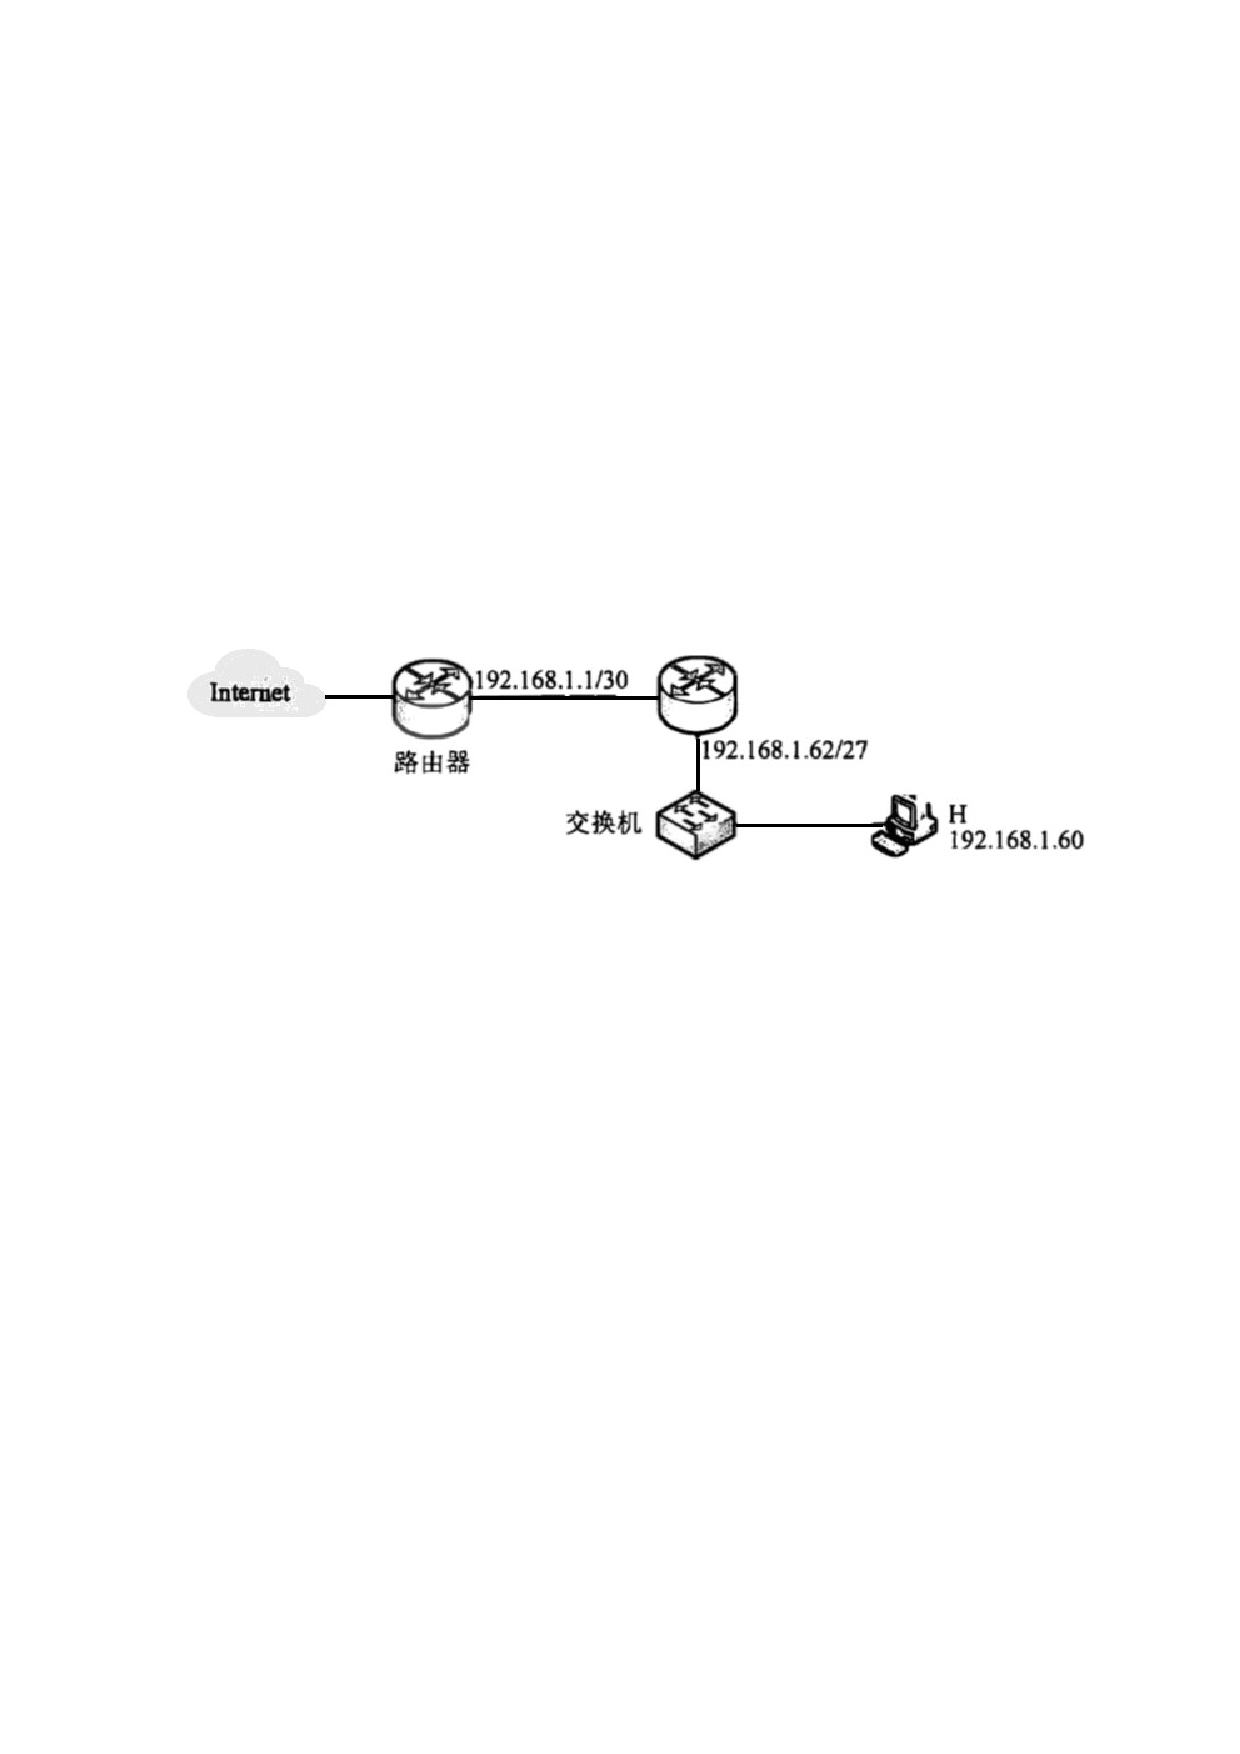
\includegraphics[width=.65\linewidth,height=.4\textheight,keepaspectratio]{../assets/figures/2022-questions-p004-b006.pdf}\end{center}

\begin{center}\begin{tabular}{>{\raggedright\arraybackslash}p{\dimexpr(\linewidth-4\tabcolsep)/2\relax}>{\raggedright\arraybackslash}p{\dimexpr(\linewidth-4\tabcolsep)/2\relax}}
\textbf{A.} 255.\allowbreak{}255.\allowbreak{}255.\allowbreak{}192, 192.\allowbreak{}168.\allowbreak{}1.\allowbreak{}1 & \textbf{B.} 255.\allowbreak{}255.\allowbreak{}255.\allowbreak{}192, 192.\allowbreak{}168.\allowbreak{}1.\allowbreak{}62\\[.35em]
\textbf{C.} 255.\allowbreak{}255.\allowbreak{}255.\allowbreak{}224, 192.\allowbreak{}168.\allowbreak{}1.\allowbreak{}1 & \textbf{D.} 255.\allowbreak{}255.\allowbreak{}255.\allowbreak{}224, 192.\allowbreak{}168.\allowbreak{}1.\allowbreak{}62\\[.35em]\end{tabular}\end{center}

37．在SDN 网络体系结构中，SDN 控制器向数据平面的SDN 交换机下发流表时所使用的接口是\_\_\_\_\_\_。


\begin{center}\begin{tabular}{>{\raggedright\arraybackslash}p{\dimexpr(\linewidth-8\tabcolsep)/4\relax}>{\raggedright\arraybackslash}p{\dimexpr(\linewidth-8\tabcolsep)/4\relax}>{\raggedright\arraybackslash}p{\dimexpr(\linewidth-8\tabcolsep)/4\relax}>{\raggedright\arraybackslash}p{\dimexpr(\linewidth-8\tabcolsep)/4\relax}}
\textbf{A.} 东向接口 & \textbf{B.} 南向接口 & \textbf{C.} 西向接口 & \textbf{D.} 北向接口\\[.35em]\end{tabular}\end{center}

38．假设主机甲和主机乙已建立一个TCP 连接，最大段长MSS = 1KB,甲一直有数据向乙发送，当甲的拥塞窗口为16KB 时，计时器发生了超时，则甲的拥塞窗口再次增长到16KB 所需要的时间至少是\_\_\_\_\_\_。


\begin{center}\begin{tabular}{>{\raggedright\arraybackslash}p{\dimexpr(\linewidth-8\tabcolsep)/4\relax}>{\raggedright\arraybackslash}p{\dimexpr(\linewidth-8\tabcolsep)/4\relax}>{\raggedright\arraybackslash}p{\dimexpr(\linewidth-8\tabcolsep)/4\relax}>{\raggedright\arraybackslash}p{\dimexpr(\linewidth-8\tabcolsep)/4\relax}}
\textbf{A.} 4RTT & \textbf{B.} 5RTT & \textbf{C.} 11RTT & \textbf{D.} 16RTT\\[.35em]\end{tabular}\end{center}

39．假设客户C 和服务器S 已建立一个TCP 连接，通信往返时间RTT=50ms，最长报文段寿命MSL = 800ms，数据传输结束后，C 主动请求断开连接。若从C 主动向S 发出FIN 段时刻算起，则C 和S 进入CLOSED 状态所需的时间至少分别是\_\_\_\_\_\_。


\begin{center}\begin{tabular}{>{\raggedright\arraybackslash}p{\dimexpr(\linewidth-8\tabcolsep)/4\relax}>{\raggedright\arraybackslash}p{\dimexpr(\linewidth-8\tabcolsep)/4\relax}>{\raggedright\arraybackslash}p{\dimexpr(\linewidth-8\tabcolsep)/4\relax}>{\raggedright\arraybackslash}p{\dimexpr(\linewidth-8\tabcolsep)/4\relax}}
\textbf{A.} 850ms，50ms & \textbf{B.} 1650ms, 50ms & \textbf{C.} 850ms, 75ms & \textbf{D.} 1650ms, 75ms\\[.35em]\end{tabular}\end{center}

40．假设主机H 通过HTTP/1.1 请求浏览某Web 服务器S 上的Web 页news408.html，news408 引用了同目录下的1 幅图像，news408.html 文件大小为1MSS（最大段长），图像文件大小为3MSS， H 访问S 的往返时间RTT=10ms，忽略HTTP 响应报文的首部开销和TCP 段传输时延。若H 已完成域名解析，则从H 请求与S 建立TCP 连接时刻起，到接收到全部内容止，所需的时间至少是\_\_\_\_\_\_。


\begin{center}\begin{tabular}{>{\raggedright\arraybackslash}p{\dimexpr(\linewidth-8\tabcolsep)/4\relax}>{\raggedright\arraybackslash}p{\dimexpr(\linewidth-8\tabcolsep)/4\relax}>{\raggedright\arraybackslash}p{\dimexpr(\linewidth-8\tabcolsep)/4\relax}>{\raggedright\arraybackslash}p{\dimexpr(\linewidth-8\tabcolsep)/4\relax}}
\textbf{A.} 30ms & \textbf{B.} 40ms & \textbf{C.} 50ms & \textbf{D.} 60ms\\[.35em]\end{tabular}\end{center}

\subsection*{二、综合应用题（第41～47小题，共70分）}

41．（13分）已知非空二叉树T的结点值均为正整数，采用顺序存储方式保存，数据结构定义如下：


\begin{Verbatim}[breaklines,breakanywhere,fontsize=\small]
typedef struct{                 // MAX_SIZE 为已定义常量
    int SqBiTNode[MAX_SIZE];    // 保存二叉树结点值的数组
    int ElemNum;                // 实际占用的数组元素个数
}SqBiTree
\end{Verbatim}

T中不存在的结点在数组SqBiTNode中用–1表示。例如，对于下图所示的两棵非空二叉树T1和T2：


\begin{center}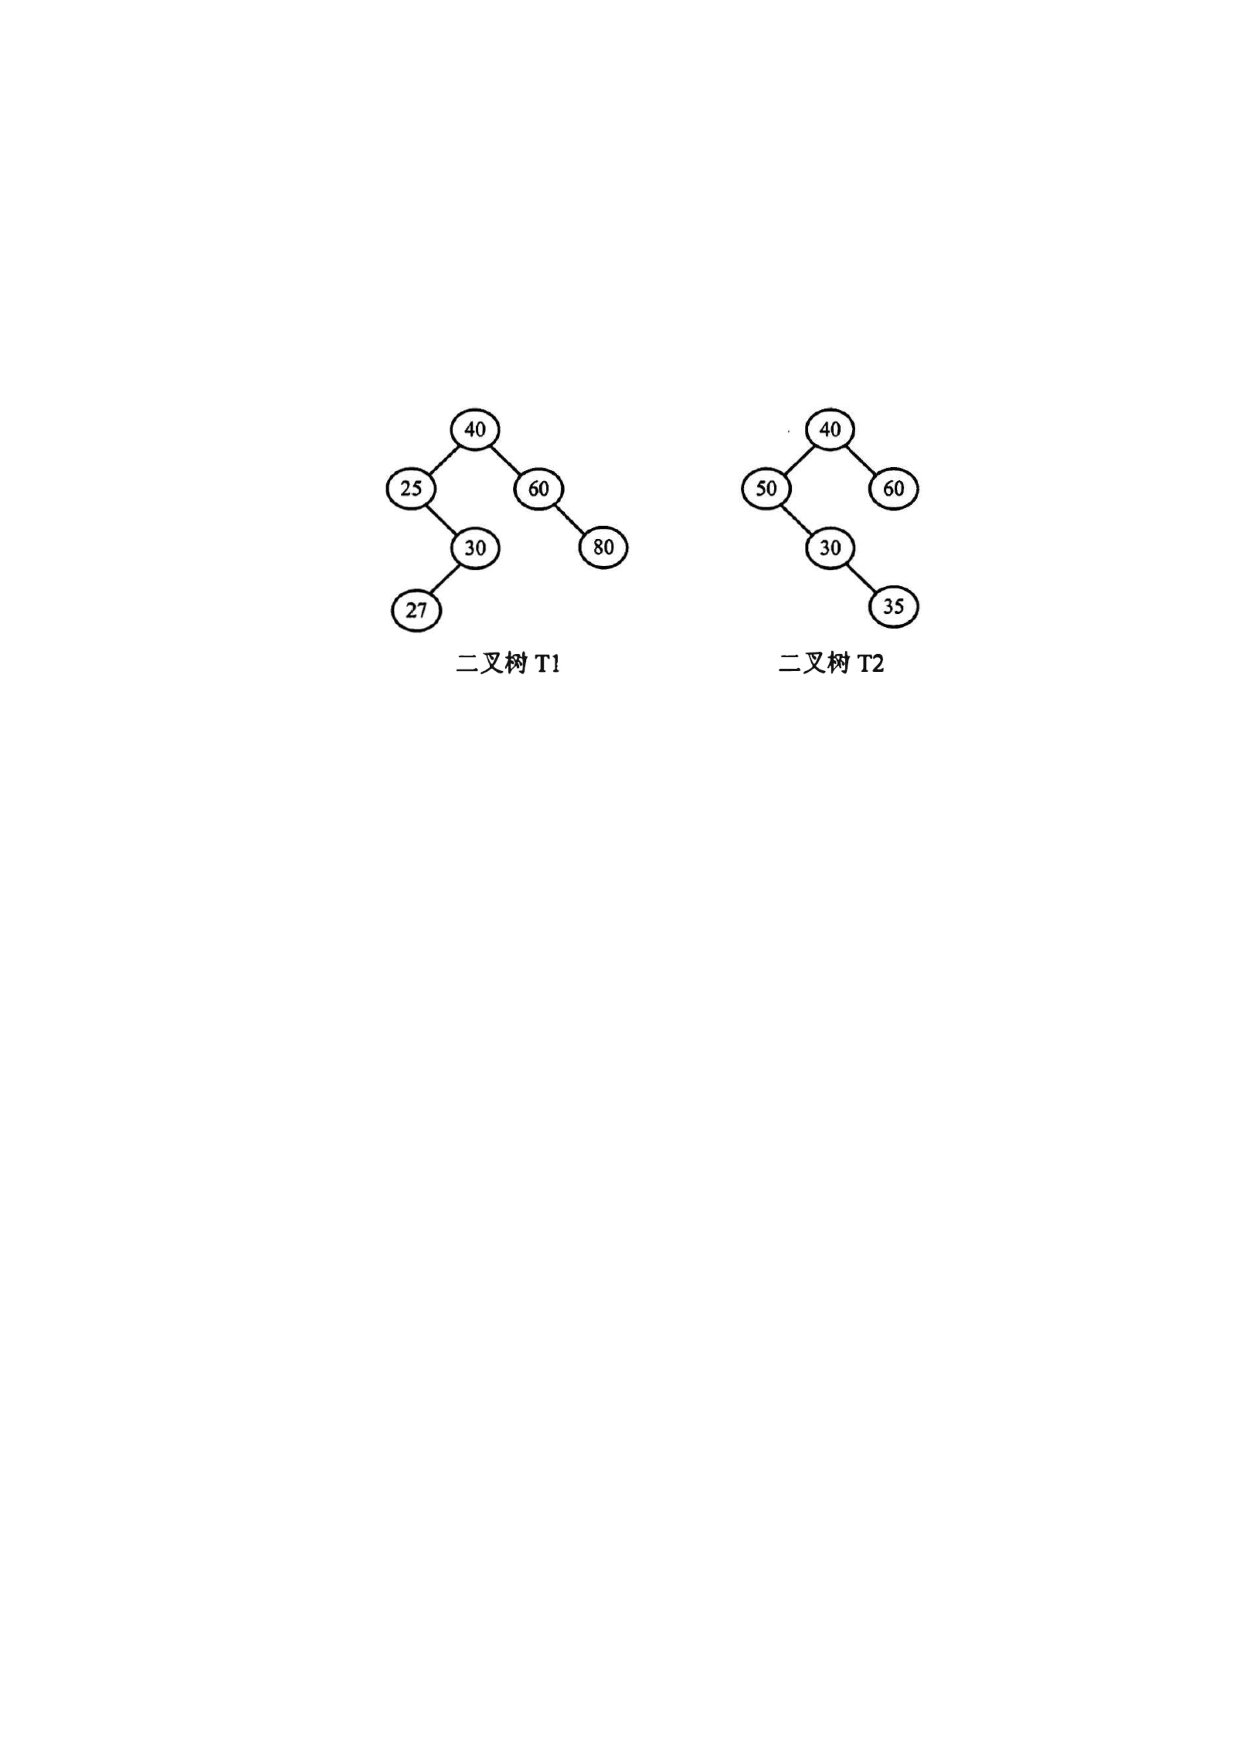
\includegraphics[width=.65\linewidth,height=.4\textheight,keepaspectratio]{../assets/figures/2022-questions-p005-b004.pdf}\end{center}

T1的存储结果如下：


\begin{center}\begin{adjustbox}{max width=\linewidth}\begin{tabular}{|c|c|c|c|c|c|c|c|c|c|c|}\hline
T1.SqBiTNode & 40 & 25 & 60 & –1 & 30 & –1 & 80 & –1 & –1 & 27\\\hline\end{tabular}\end{adjustbox}\end{center}

T1.ElemNum = 10。T2的存储结果如下：


\begin{center}\begin{adjustbox}{max width=\linewidth}\begin{tabular}{|c|c|c|c|c|c|c|c|c|c|c|c|}\hline
T2.SqBiTNode & 40 & 50 & 60 & –1 & 30 & –1 & –1 & –1 & –1 & –1 & 35\\\hline\end{tabular}\end{adjustbox}\end{center}

T1.ElemNum = 11。请设计一个尽可能高效的算法，判断一棵采用这种方式存储的二叉树是否为二叉搜索树，若是，则返回true，否则，返回false。要求：（1）给出算法的基本设计思想。（2）根据设计思想，采用C或C++语言描述算法，关键之处给出注释。


42．（10分）现有\(\displaystyle n\)（\(\displaystyle n>100000\)）个数保存在一维数组M中，需要查找M中最小的10个数，请回答下列问题：（1）设计一个完成上述查找任务的算法，要求平均情况下的比较次数尽可能少，简述算法思想（不需要程序实现）。（2）说明你所设计的算法平均情况下的时间复杂度和空间复杂度。


43．（15分）某CPU中部分数据通路如题43图所示，其中，GPRs为通用寄存器组；FR为标志寄存器，用于存放ALU产生的标志信息；带箭头虚线表示控制信号，如控制信号Read、Write分别表示主存读、主存写，MDRin表示内部总线上数据写入MDR，MDRout表示MDR的内容送内部总线。


\begin{center}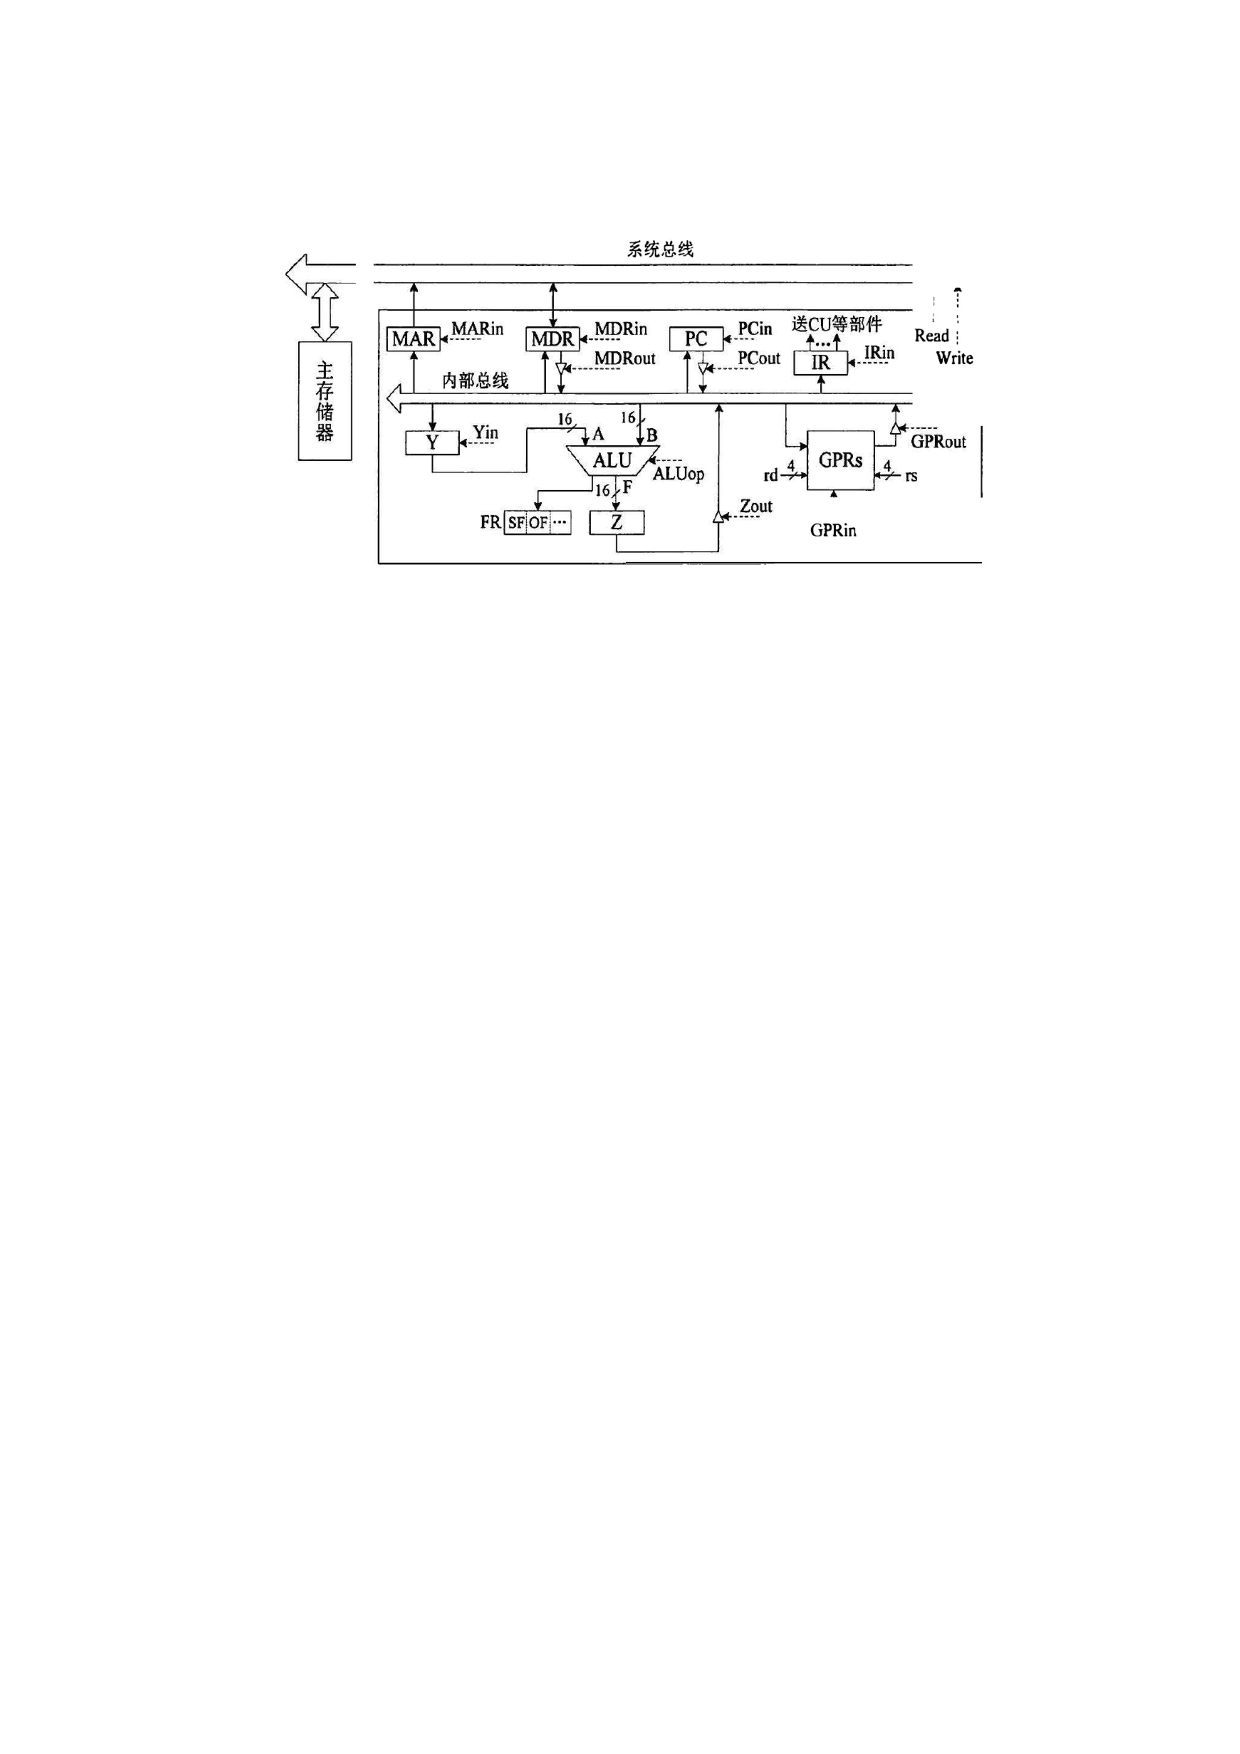
\includegraphics[width=.65\linewidth,height=.4\textheight,keepaspectratio]{../assets/figures/2022-questions-p007-b001.pdf}\end{center}

请回答下列问题：（1）设ALU的输入端A、B及输出端F的最高位分别为\(\displaystyle A_{15}\)、\(\displaystyle B_{15}\)及\(\displaystyle F_{15}\)，FR中的符号标志和溢出标志分别为SF和OF，则SF的逻辑表达式是什么？A加B、A减B时OF的逻辑表达式分别是什么？要求逻辑表达式的输入变量为\(\displaystyle A_{15}\)、\(\displaystyle B_{15}\)及\(\displaystyle F_{15}\)。（2）为什么要设置暂存器Y和Z？（3）若GPRs的输入端rs、rd分别为所读、写的通用寄存器的编号，则GPRs中最多有多少个通用寄存器？rs和rd来自图中的哪个寄存器？已知GPRs内部有一个地址译码器和一个多路选择器，rd应连接地址译码器还是多路选择器？（4）取指令阶段（不考虑PC增量操作）的控制信号序列是什么？若从发出主存读命令到主存读出数据并传送到MDR共需5个时钟周期，则取指令阶段至少需要几个时钟周期？（5）图中控制信号由什么部件产生？图中哪些寄存器的输出信号会连到该部件的输入端？


44．（8 分）假设某磁盘驱动器中有4 个双面盘片，每个盘面有20000 个磁道，每个磁道有500 个扇区，每个扇区可记录512 字节的数据，盘片转速为7200RPM（转/分），平均寻道时间为5ms。请回答下列问题。 （1）每个扇区包含数据及其地址信息，地址信息分为3 个字段。这3 个字段的名称各是什么？ 对于该磁盘，各字段至少占多少位？ （2）一个扇区的平均访问时间约为多少？ （3）若采用周期挪用DMA 方式进行磁盘与主机之间的数据传送，磁盘控制器中的数据缓冲区大小为64 位，则在一个扇区读写过程中，DMA 控制器向CPU 发送了多少次总线请求？若CPU 检测到DMA 控制器的总线请求信号时也需要访问主存，则DMA 控制器是否可以获得总线使用权？为什么？


45．（7分）某文件系统的磁盘块大小为4KB，目录项由文件名和索引结点号构成，每个索引结点占256字节，其中包含直接地址项10个，一级、二级和三级间接地址项各1个，每个地址项占4字节。该文件系统中子目录stu的结构如题45（a）图所示，stu包含子目录course和文件doc，course子目录包含文件course1和course2。各文件的文件名、索引结点号、占用磁盘块的块号如题45（b）图所示。


\begin{center}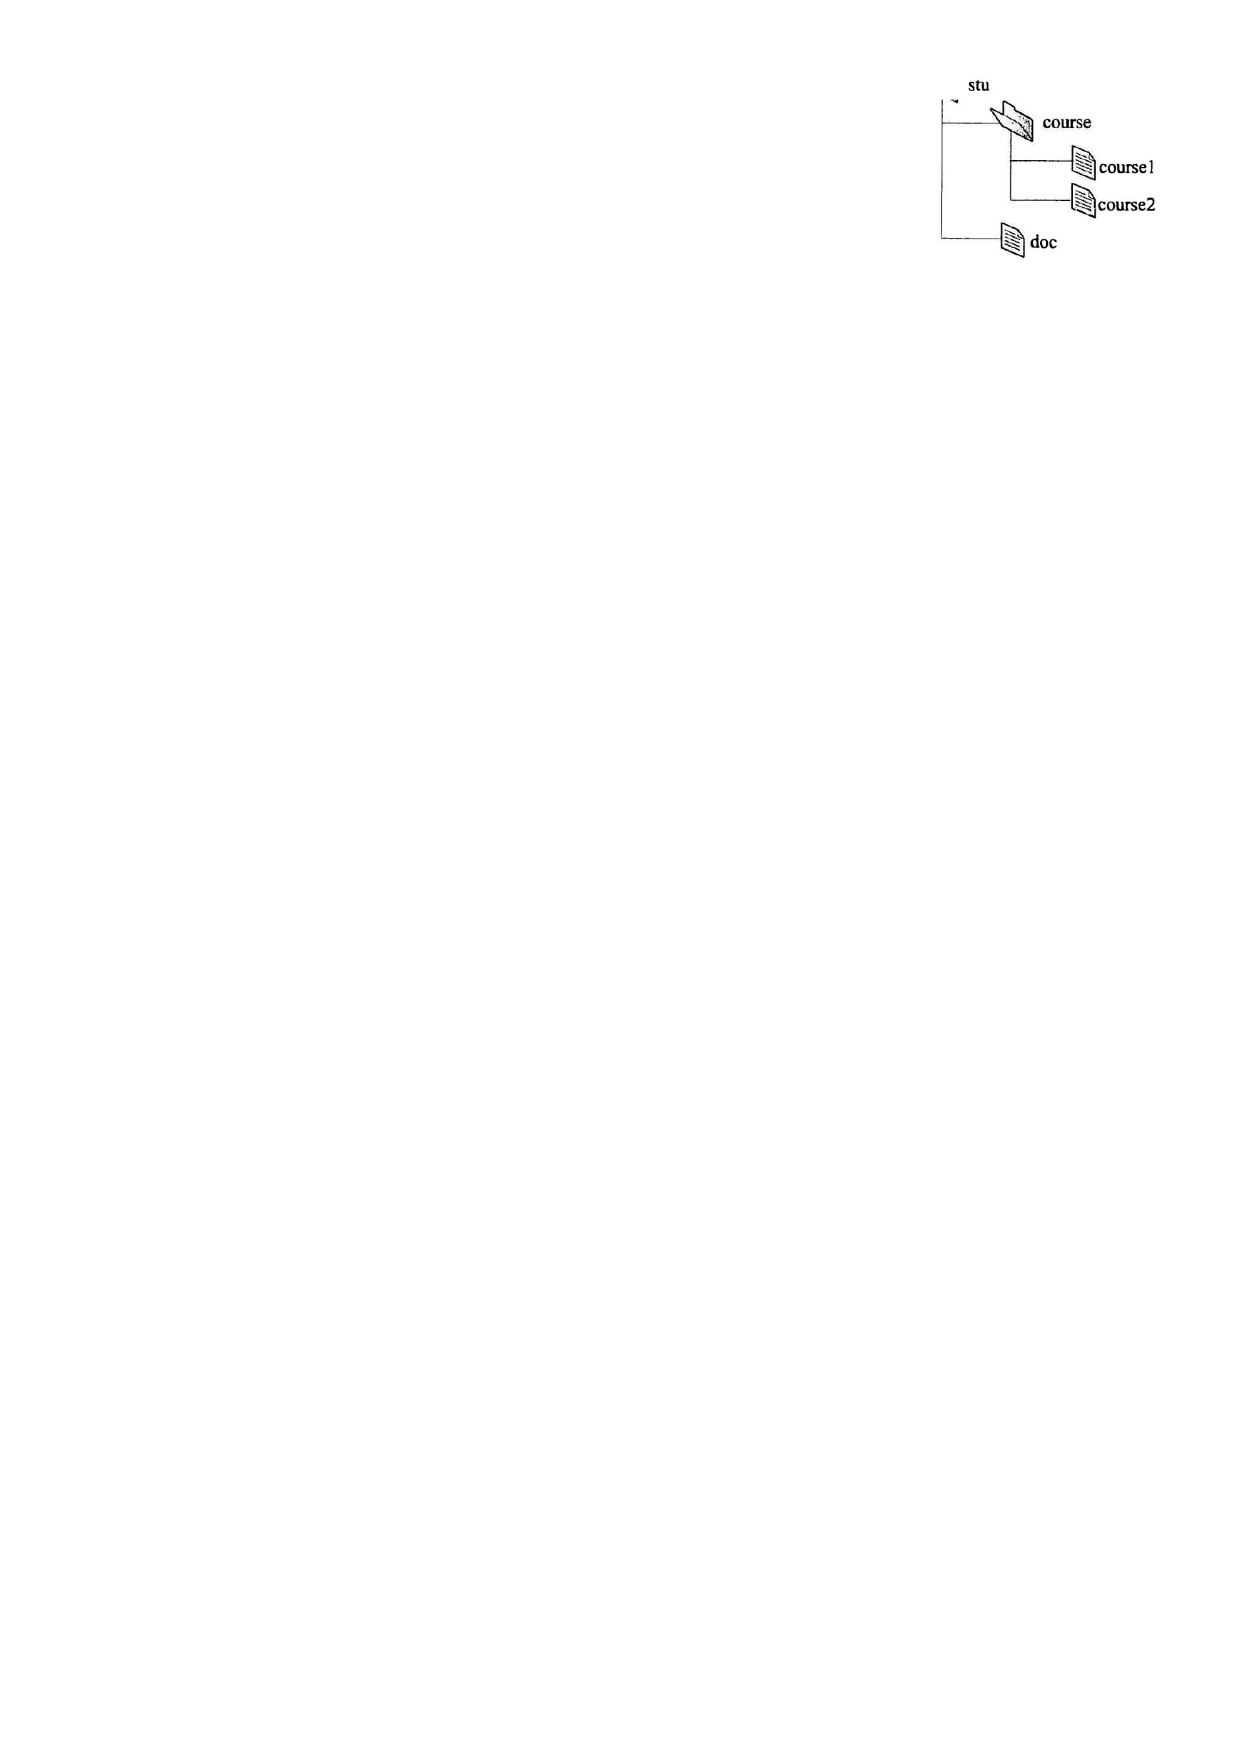
\includegraphics[width=.65\linewidth,height=.4\textheight,keepaspectratio]{../assets/figures/2022-questions-p009-b001.pdf}\end{center}

\begin{center}\begin{adjustbox}{max width=\linewidth}\begin{tabular}{|>{\raggedright\arraybackslash}p{\dimexpr(\linewidth-6\tabcolsep-4\arrayrulewidth)/3\relax}|>{\raggedright\arraybackslash}p{\dimexpr(\linewidth-6\tabcolsep-4\arrayrulewidth)/3\relax}|>{\raggedright\arraybackslash}p{\dimexpr(\linewidth-6\tabcolsep-4\arrayrulewidth)/3\relax}|}\hline
文件名 & 索引结点号 & 磁盘块号\\\hline
stu & 1 & 10\\\hline
course & 2 & 20\\\hline
course1 & 10 & 30\\\hline
course2 & 100 & 40\\\hline
doc & 10 & x\\\hline\end{tabular}\end{adjustbox}\end{center}

请回答下列问题：（1）目录文件stu中每个目录项的内容是什么？（2）文件doc占用的磁盘块的块号x的值是多少？（3）若目录文件course的内容已在内存，则打开文件course1并将其读入内存，需要读几个磁盘块？说明理由。（4）若文件course2的大小增长到6MB，则为了存取course2需要使用该文件索引结点的哪几级间接地址项？说明理由。


46．（8分）某进程的两个线程T1和T2并发执行A、B、C、D、E和F共6个操作，其中T1执行A、E和F，T2执行B、C和D。题46图表示上述6个操作的执行顺序所必须满足的约束；C在A和B完成后执行，D和E在C完成后执行，F在E完成后执行。请使用信号量的wait()、signal()操作描述T1和T2之间的同步关系，并说明所用信号量的作用及其初值。


\begin{center}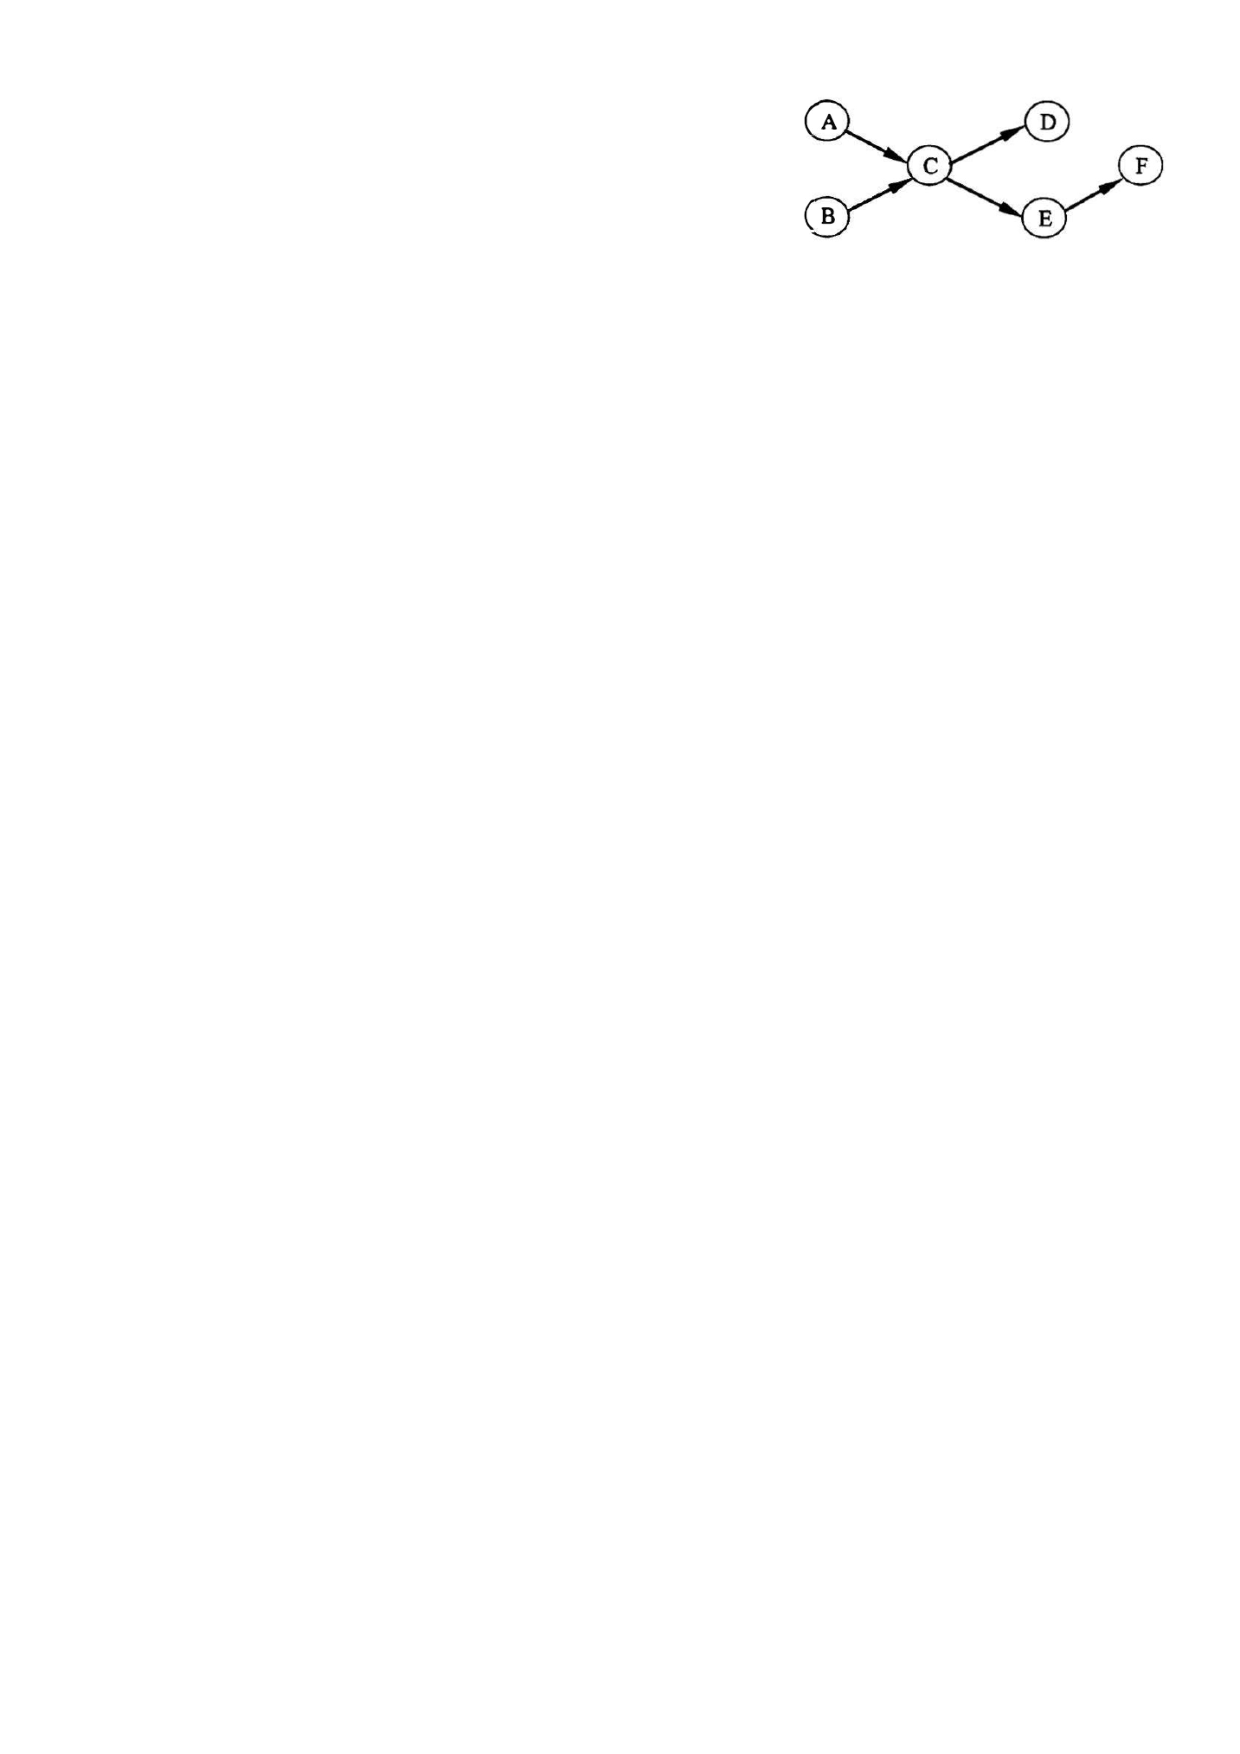
\includegraphics[width=.65\linewidth,height=.4\textheight,keepaspectratio]{../assets/figures/2022-questions-p010-b001.pdf}\end{center}

47．（9分）网络拓扑如题47图所示，R为路由器，S为以太网交换机，AP是802.11接入点，路由器的E0接口和DHCP服务器的IP地址配置如图中所示；H1与H2属于同一个广播域，但不属于同一个冲突域；H2和H3属于同一个冲突域；H4和H5已经接入网络，并通过DHCP动态获取了IP地址。现有路由器、100BaseT以太网交换机和100BaseT集线器（Hub）三类设备各若干台。


\begin{center}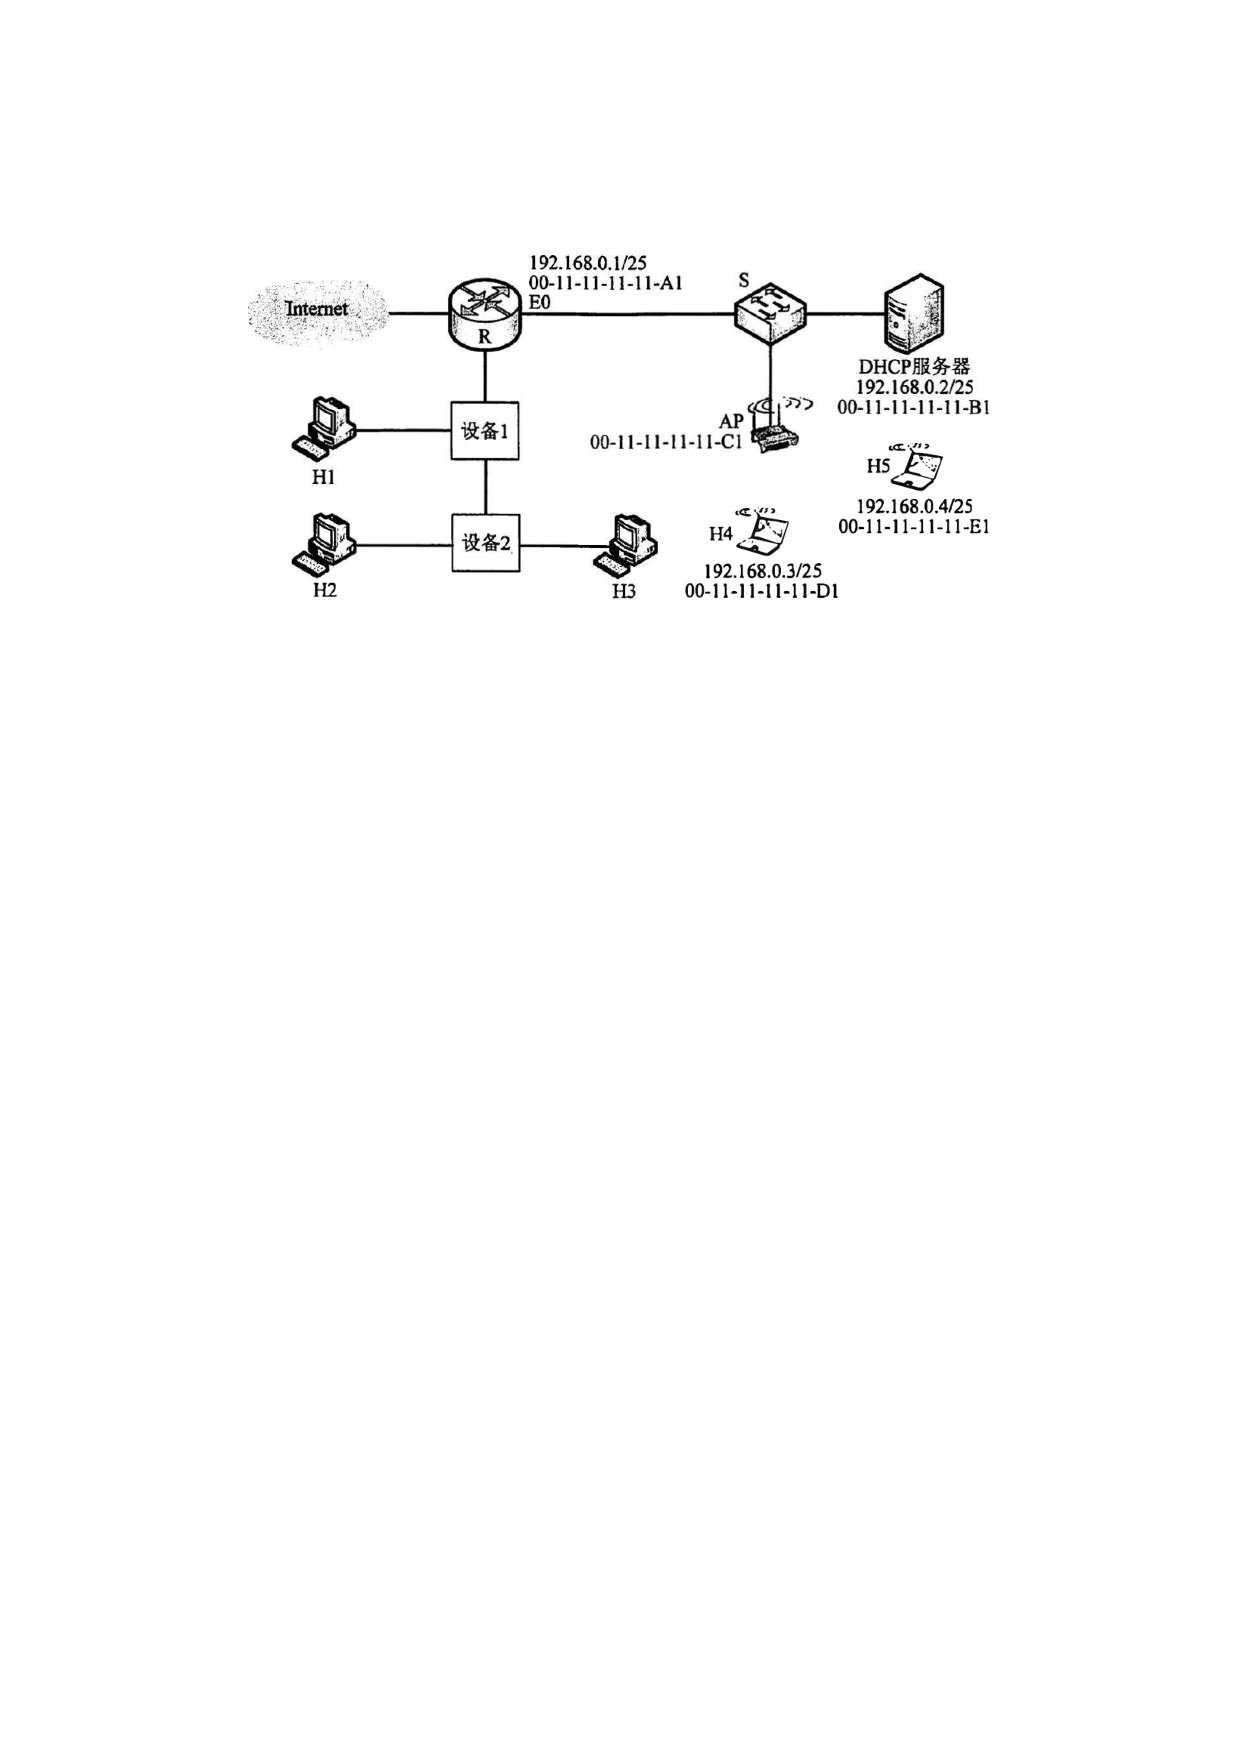
\includegraphics[width=.65\linewidth,height=.4\textheight,keepaspectratio]{../assets/figures/2022-questions-p011-b001.pdf}\end{center}

请回答下列问题：（1）设备1和设备2应该分别选择哪类设备？（2）若信号传播速度为\(\displaystyle 2\times10^8\,\mathrm{m/s}\)，以太网最小帧长为64B，信号通过设备2时会产生额外的\(\displaystyle 1.51\,\mu\mathrm{s}\)时间延迟，则H2与H3之间可以相距的最远距离是多少？（3）在H4通过DHCP动态获取IP地址过程中，H4首先发送了DHCP报文M，M是哪种DHCP报文？路由器E0接口能否收到封装M的以太网帧？S向DHCP服务器转发的封装M的以太网帧的目的MAC地址是什么？（4）若H4向H5发送一个IP分组P，则H5收到的封装P的802.11帧的地址1、地址2和地址3分别是什么？

\end{document}
